 \documentclass[11pt]{beamer}
 \usetheme{Madrid}
 \usepackage[utf8]{inputenc}
 \usepackage[french]{babel}
 \usepackage[T1]{fontenc}
 \usepackage{amsmath}
 \usepackage{amsfonts}
 \usepackage{amssymb}
 \usepackage{graphicx}
 \usepackage{algorithm2e}
 \author{\textbf{Présenté par:} \\ \textit{Tafsir GNA} \\ \textbf{Supervisé par:} \\ \textit{Dr Ing. Vinasétan Ratheil HOUNDJI \\ \& \\ Professeur Mahouton Norbert HOUNKONNOU}}
 \title{Résolution du \emph{Pigment Sequencing Problem} avec les algorithmes génétiques}
 %\setbeamercovered{transparent} 
 %\setbeamertemplate{navigation symbols}{} 
 %\logo{} 
\institute{Institut de Formation et de Recherche en Informatique (IFRI)} 
 %\date{} 
 %\subject{} 
 \begin{document}
 
 \begin{frame}
	\hbox to \textwidth
 	{
 		
\includegraphics[scale=0.2]{img/ifri_logo.png}
 		\hfill
 		\texttt{Mémoire de master en Informatique}
 		\hfill
 		
\includegraphics[scale=0.2]{img/uac_logo.png}
 	}
	\titlepage
\end{frame} 


 
 % Page de sommaire
 \begin{frame}
 \frametitle{Sommaire}
 \setcounter{tocdepth}{1}
 \tableofcontents
 \end{frame}

 \section{Introduction}
 \begin{frame}
 \frametitle{Introduction}
 \framesubtitle{Le dimensionnement de lots}
 	\begin{figure}
   \begin{minipage}[c]{.46\linewidth}
      \includegraphics[scale=.7]{img/image_intro1.png}
   \end{minipage} \hfill
   \begin{minipage}[c]{.46\linewidth}
      \includegraphics[scale=.6]{img/image_intro2.png}
   \end{minipage}
\end{figure}
 \end{frame} 
 
 \begin{frame}
 \frametitle{Introduction}
 \framesubtitle{Les algorithmes génétiques}
 	\begin{figure}
   \begin{minipage}[c]{.46\linewidth}
      \includegraphics[scale=.7]{img/image_gene1.png}
   \end{minipage} \hfill
   \begin{minipage}[c]{.46\linewidth}
      \includegraphics[scale=.7]{img/image_gene2.png}
   \end{minipage}
\end{figure}
 \end{frame} 
 
 % Etat de l'art
 \section{Etat de l'art et formulation du problème}
    
 \subsection{Le "Pigment Sequencing Problem" (PSP)}
 
 \begin{frame}
 	\begin{minipage}[c]{.46\linewidth}
      \Large{\emph{\textbf{Pigment Sequencing Problem (PSP) }}}
   \end{minipage} \hfill
   \begin{minipage}[c]{.46\linewidth}
		\includegraphics[scale=.6]{img/reflexion.png}
   \end{minipage}
\end{frame}  
 
 \begin{frame}
 \transsplitverticalin
 \frametitle{Le "Pigment Sequencing Problem" (PSP)}
 \framesubtitle{Description}
 
 	Objectif:
    \begin{itemize}
    	\item<2-> trouver un plan de production de plusieurs articles à partir d’une
machine dont la capacité de production est limité à un article par période;
		\vspace*{.5cm}
    	\item<3-> minimisant les coûts de stockage et de transition;
    	\vspace*{.5cm}
    	\item<4-> les demandes sont normalisées et donc binaires.
    \end{itemize}
 \end{frame} 
 
 \begin{frame}
 \transboxout
 \frametitle{Le "Pigment Sequencing Problem" (PSP)}
 \framesubtitle{Modèle mathématique du PSP}
 	\begin{eqnarray}
		min \sum_{i,j,t} q^{i,j}\chi_{t}^{i,j} + \sum_{i,t} h^{i} s_{t}^{i} \\
		s_{0}^{i} = 0, \forall i \\
		x_{t}^{i} + s_{t-1}^{i} = d_{t}^{i} + s_{t}^{i}, \forall i,t \\
		x_{t}^{i} \leq y_{t}^{i}, \forall i,t \\
		\sum_{i} y_{t}^{i} = 1 , \forall t \\
		\chi_{t}^{i,j} = y_{t-1}^{i} + y_{t}^{j} - 1, \forall i,j,t \\
		x,y,\chi \in \{0,1\}, s \in \mathbb{N}, i \in \{0..NI\}, t \in \{1..NT\}
	\end{eqnarray}
 \end{frame} 
 
 \begin{frame}
 \transreplace
 \frametitle{Le "Pigment Sequencing Problem" (PSP)}
 \framesubtitle{Etat de l'art} 
 
 	Travaux:
    \begin{itemize}
    	\item Pochet et Wolsey et formulations MIP du DLSP;
    	\item<2->Houndji et al et programmation par contraintes;
    	\item<3->Ceschia et al. et le recuit simulé;
    	\item<4-> ...
    	\item<5-> ...
    	\item<6-> \LARGE{\textcolor{red}{Tafsir Gna et Algorithmes génétiques.}}
    \end{itemize}
 \end{frame} 
 
 \begin{frame}
 	\begin{minipage}[c]{.46\linewidth}
      \Large{\emph{\textbf{Les algorithmes génétiques (AGs)}}}
   \end{minipage} \hfill
   \begin{minipage}[c]{.46\linewidth}
		\includegraphics[scale=.6]{img/reflexion.png}
   \end{minipage}
\end{frame}  


\begin{frame}
\frametitle{Les algorithmes génétiques}
\begin{figure}
   \begin{minipage}[c]{.46\linewidth}
      \includegraphics[scale=.5]{img/algo_gene1.png}
   \end{minipage} \hfill
   \begin{minipage}[c]{.46\linewidth}
      \includegraphics[scale=.5]{img/algo_gene2.png}
   \end{minipage}
 \end{figure}
\end{frame} 

\begin{frame}
\frametitle{Les algorithmes génétiques}
\framesubtitle{Fonctionnement}
\begin{figure}
      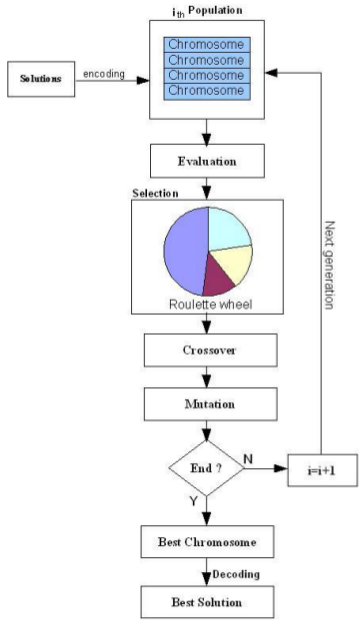
\includegraphics[scale=.3]{img/genetic_algo_flowchart.png}
      \caption{Diagramme d'un algorithme génétique standard}
	  \label{fig:genetic_algo_flowchart}
 \end{figure}
\end{frame} 

 \begin{frame}
 \transsplitverticalin
 \frametitle{Les algorithmes génétiques}
 \framesubtitle{Les algorithmes génétiques parallèles}
	%\begin{figure}
	De la gauche vers la droite dans l'ordre : master-slave, coarsed-grained, fine-grained
	\begin{tabular}{ccc}
		%\begin{figure}
		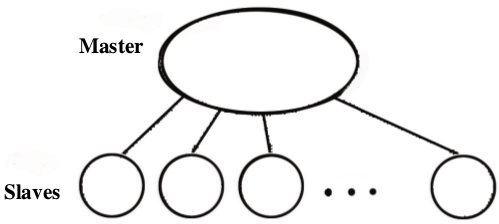
\includegraphics[scale=.3]{img/master_slave_ga.png} 
		&
		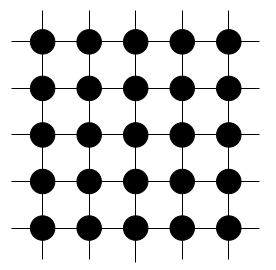
\includegraphics[scale=.3]{img/fine_grained_fig.png}
    	&	
   		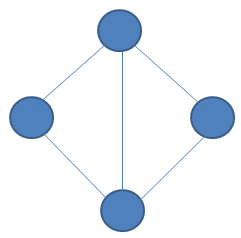
\includegraphics[scale=.3]{img/topology_fig.png} 
   		%\caption{}	
   		%\end{figure}
	\end{tabular}
	%\end{figure}
	
 \end{frame}
 
 \begin{frame}
 \frametitle{Les algorithmes génétiques}
 \framesubtitle{Hiérarchisation entre les algorithmes génétiques parallèles}
 		\begin{figure}
   		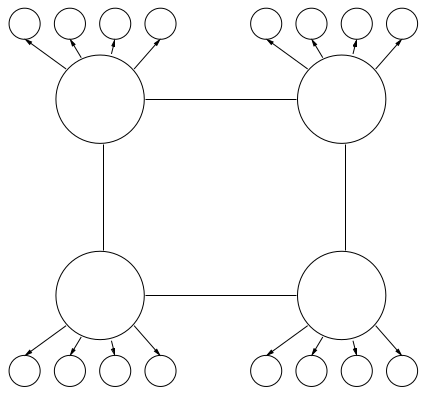
\includegraphics[scale=.15]{img/hierarchical_gene1_fig.png} 
   		\caption{HCM-PGA}
   		\end{figure}
   		\hfill
   		\begin{figure}
   		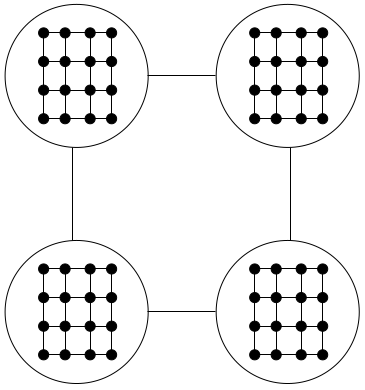
\includegraphics[scale=.15]{img/hierar_fine_grained_fig.png}
   		\caption{HCM-PGA}
   		\end{figure}
 	
 \end{frame}
 
 % Matériel et Méthodes
 \section{Méthodes et Solutions}
 
 \begin{frame}
 \transsplitverticalin
 	\frametitle{Méthodes et solutions}
 	\begin{center}
 		\LARGE{\texttt{Méthodes et solutions}}
 	\end{center}
 \end{frame}  
 
 \subsection{Aspects généraux aux deux méthodes de recherche proposées}
 
 \begin{frame}
 \frametitle{Aspects généraux aux deux méthodes de recherche proposées}
 \framesubtitle{Axes d'implémentation}
 	\begin{itemize}
 		\item Comment représenter t-on nos chromosomes ?
 		\item<2-> Comment initialise t-on notre population ?
 		\item<3-> Comment sélectionne t-on nos chromosomes parents ?
 		\item<4-> Comment croise t-on nos chromosomes parents ?
 		\item<5-> ...
 	\end{itemize}
 \end{frame} 
 
 \begin{frame}
 \frametitle{Aspects généraux aux deux méthodes de recherche proposées}
 \framesubtitle{Représentation génétique}
	
	\begin{center}
		$ch_{Tn} = \{(I_{T1}),..., (I_{T2}),..., (I_{T3}), (I_{T4}),...,(I_{T(n-1)}),...,  (I_{Tn})\}$ \\
	\end{center}
	\hspace*{.5cm} où $ch_{Tn}$ est un chromosome dont l'horizon de planification est de $Tn$ périodes et $I_{Ti}$ est la variable entière qui indique l'article produit à la période \emph{Ti}.  \\
	
	\hspace*{.5cm} \textsl{\textbf{Illustration}} avec les demandes $D_{I1} = (0,1,0,0,1)$ et $D_{I2} = (1,0,0,0,1)$ 
 \begin{figure}[!h]
		\begin{center}
			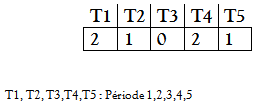
\includegraphics[scale=.5]{img/adopt_gene_repr.png}
			\caption{Représentation génétique adoptée}
			\label{fig:adopt_gene_repr}
		\end{center}
 \end{figure}
 \end{frame}
 
 \begin{frame}
 \transsplithorizontalout
 \frametitle{Aspects généraux aux deux méthodes de recherche proposées}
 \framesubtitle{Initialisation}
	\begin{figure}[!h]
		\begin{center}
			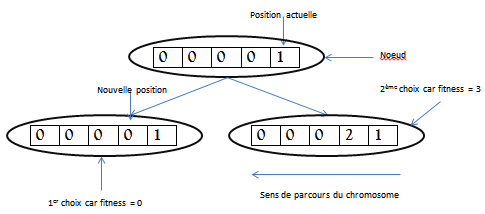
\includegraphics[scale=.5
			]{img/hill_climbing_fig.png}
			\caption{Schéma illustratif de l'application de l'algorithme du Hill climbing à une instance de PSP}
			%\label{fig:adopt_gene_repr}
		\end{center}
 \end{figure}
	
 \end{frame}
 
  \begin{frame}
 \frametitle{Aspects généraux aux deux méthodes de recherche proposées}
 \framesubtitle{Evaluation}
 
 \textbf{Evaluation}
	\begin{figure}[!h]
		\begin{center}
			\includegraphics[scale=.5
			]{img/eval_fig.png}
			\caption{Schéma illustratif de la méthode d'évaluation utilisée}
			%\label{fig:adopt_gene_repr}
		\end{center}
 \end{figure}
	
 \end{frame} 
 
 \begin{frame}
 \frametitle{Aspects généraux aux deux méthodes de recherche proposées}
 \framesubtitle{Sélection}
	
	\textbf{Sélection}
	\begin{figure}[!h]
		\begin{center}
			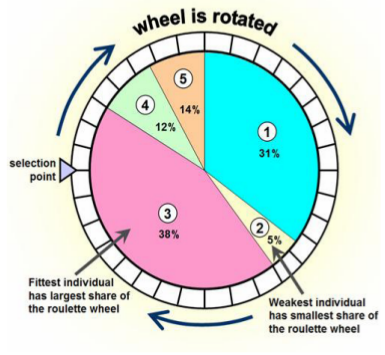
\includegraphics[scale=.5
			]{img/wheel_fig.png}
			\caption{Schéma illustratif de la méthode de \emph{roulette wheel}}
			%\label{fig:adopt_gene_repr}
		\end{center}
 \end{figure}
	
 \end{frame}
 
 \begin{frame}
 \frametitle{Aspects généraux aux deux méthodes de recherche proposées}
 \framesubtitle{Croisement}
	
	\textbf{Croisement}
	\begin{figure}[!h]
		\begin{center}
			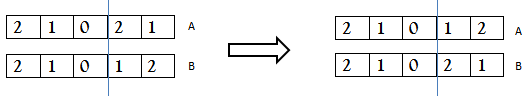
\includegraphics[scale=.5
			]{img/cross_over_fig.png}
			\caption{Schéma illustratif de la méthode de croisement utilisée}
			%\label{fig:adopt_gene_repr}
		\end{center}
 \end{figure}
	
 \end{frame}
 
 \begin{frame}
 \frametitle{Aspects généraux aux deux méthodes de recherche proposées}
 \framesubtitle{Fonction de faisabilité}
	
	\textbf{Principe:}
	\vspace*{.5cm}
    \begin{itemize}
    	\item Réduction du surplus de production;
    	\vspace*{.5cm}
    	\item<2-> Production d'articles à des périodes données afin de combler une sous-production.
    \end{itemize}
	
 \end{frame} 
 
 \begin{frame}
 \frametitle{Aspects généraux aux deux méthodes de recherche proposées}
 \framesubtitle{Mutation}
	
	\textbf{Mutation}
	\begin{figure}[!h]
		\begin{center}
			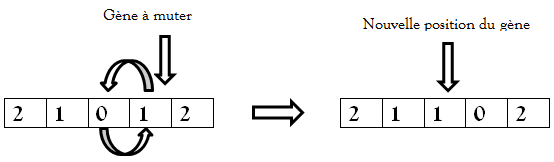
\includegraphics[scale=.5
			]{img/mutation_fig.png}
			\caption{Schéma illustratif de la méthode de mutation utilisée}
			%\label{fig:adopt_gene_repr}
		\end{center}
 \end{figure}
	
 \end{frame}
 
 \begin{frame}
 \frametitle{Aspects généraux aux deux méthodes de recherche proposées}
 \framesubtitle{Terminaison}
	
	\textbf{Deux critères de terminaison}
	\vspace*{.5cm}
	\begin{itemize}
		\item Convergence de la population sur une solution;
		\vspace*{.5cm}
		\item<2-> Absence de meilleures solutions à partir de celle trouvée.
		\vspace*{.5cm}
		\item<3-> Hybridation
	\end{itemize}
	
 \end{frame}
 
 \subsection{Méthodes de recherche proposées}
 
 \begin{frame}
 \frametitle{Méthodes de recherche proposées}
 \framesubtitle{Algorithmes génétiques parallèles et hiérarchiques coarse-grained et
master-slave / Algorithmes génétiques parallèles et hiérarchiques coarse-grained et
fine-grained}
	
	Problématiques :
	\begin{itemize}
		\item Fréquence de migration;
		\item Choix et nombre de migrants;
		\item Topologie de connexions;
		\item Méthode d’intégration des migrants;
	\end{itemize}
	
 \end{frame} 
 
 % Résultats et discussion
 \section{Résultats et discussion}
 
 \begin{frame}
 	\frametitle{Matériel et Méthodes}
 	\begin{center}
 		\LARGE{\texttt{Résultats et discussion}}
 	\end{center}
 \end{frame}   
 
 
 \subsection{Données et paramètres de test}
 \begin{frame}
 \frametitle{Résultats et discussion}
 \framesubtitle{Données et paramètres de test}
 \begin{itemize}
					\item[-] Taille de la population : 25 individus par processus ;
			        \item[-] Probabilité de mutation : 5\%;
			        \item[-] Probabilité de croisement : 80\%;
			        \item[-] Nombre de migrants : 1 individu;
		 	        \item[-] Nombre de processus esclaves : 2 processus (cas du HCM-PGA);
			        \item[-] Nombre de processus principaux : 2 processus (cas du HFC-PGA);
			        \item[-] Nombre de générations avant migration : 0 génération (la migration intervient après une convergence).
				\end{itemize}
 \end{frame}
 
 \subsection{Résultats expérimentaux des algorithmes génétiques parallèles hiérarchiques fine-grained et coarse-grained}
 
 \begin{frame}
 \frametitle{Résultats expérimentaux des algorithmes génétiques parallèles hiérarchiques fine-grained et coarse-grained}
 \framesubtitle{HFC-PGA et CP}
 \begin{figure}[!h]
		\begin{center}
			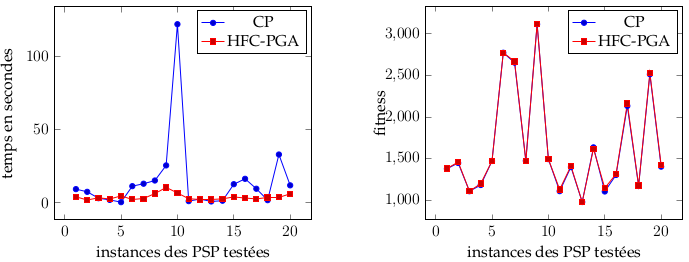
\includegraphics[scale=.4
			]{img/cp_hfc.png}
			\caption{Résultats expérimentaux HFC-PGA et CP}
		\end{center}
 \end{figure}
 \end{frame}
 
 \subsection{Résultats expérimentaux des algorithmes génétiques parallèles hiérarchiques master-slave et coarse-grained}
 
 \begin{frame}
 \frametitle{Résultats expérimentaux des algorithmes génétiques parallèles hiérarchiques master-slave et coarse-grained}
 \framesubtitle{HCM-PGA et SA}
 \begin{figure}[!h]
		\begin{center}
			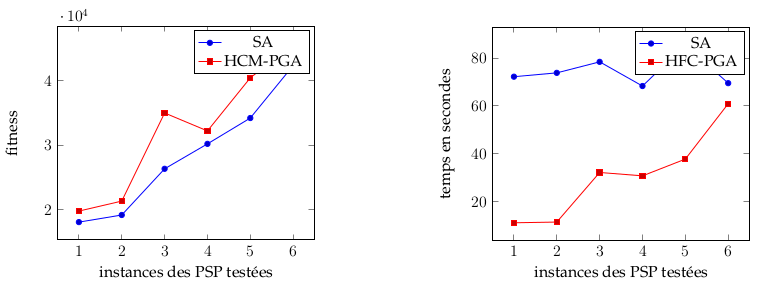
\includegraphics[scale=.4
			]{img/sa_hcm.png}
			\caption{Résultats expérimentaux HCM-PGA et SA}
		\end{center}
 \end{figure}
 \end{frame}
 
 \begin{frame}
  \frametitle{Test}
 	\begin{center}
 		\LARGE{\texttt{Test}}
 	\end{center}
 \end{frame} 
 
 % Conclusion
 \section{Conclusion et perspectives}
 \begin{frame}
  \frametitle{Conclusion et Perspectives}
 	\begin{center}
 		\LARGE{\texttt{Conclusion et perspectives}}
 	\end{center}
 \end{frame}
 
 \begin{frame}
 	\begin{figure}[!h]
		\begin{center}
			\includegraphics[scale=.4
			]{img/merci.png}
			%\caption{Schéma illustratif de la méthode de mutation utilisée}
			%\label{fig:adopt_gene_repr}
		\end{center}
 \end{figure}
 \end{frame}
 
% \begin{frame}{•}
% 
% \end{frame}
 
 \end{document}